\documentclass[main.tex]{subfiles}

\begin{document}
	
\section{Постановка задачи}
Поставлена проблема двумерной минимизации:
\begin{equation}\label{eq:problem}
f(x_1, x_2)=x_1^2+x_2^2+cos(x_1+3x_2)-x_1+2x_2 \rightarrow \min_{x_1, x_2}
\end{equation}
Необходимо:
\begin{itemize}
	\item Решить задачу (\ref{eq:problem}) методом наискорейшего спуска;
	\item Доказать сходимость метода наискорейшего спуска применительно к данной функции;
	\item Обосновать выбор условия окончания вычислений для метода одномерной минимизации по соответствующему условию градиентного метода, показать справедливость вывода в ходе вычислительного эксперимента при точности градиентного метода 0.01;
	\item Решить ту же задачу методом Ньютона второго порядка.
\end{itemize}

\section{Обоснование применимости методов}
Оценим сходимость метода наискорейшего спуска, используя теорему 1.1 \cite{boldirev}. Покажем, что функция \ref{eq:problem} подчиняется следующим условиям:\\
\begin{gather} % amsmath package
\label{eq:convex} 
f(x) \in C^1(\mathds{R})\\
\label{eq:bounded}
\exists m \in \mathds{R}: m \le f(x) \forall x \in \mathds{R}^2 \\
\label{eq:lipshitz}
\exists L \in \mathds{R}: \norm{\nabla f(x) - \nabla f(y)} \le L\norm{x-y} \forall x,y \in \mathds{R}^2
\end{gather}

Для функции, удовлетворяющей вышеперечисленным условиям, в случае итерационной схемы градиентного спуска с параметром $eps > 0$, характеризующим окончание вычислений, теорема утверждает следующее: 
если номер шага $k\rightarrow \infty$, то выполняется условие выхода $\norm{\nabla f(x_k)}^2 \le eps$  (иначе говоря, при выполнении условий (\ref{eq:convex}), (\ref{eq:bounded}), (\ref{eq:lipshitz}) рано или поздно градиентный спуск -- в частности, метод наискорейшего спуска -- закончит работу).\\
Проверим выполнение условий.\\
\begin{gather*}
\frac{\partial f}{\partial x_1} = 2x_1 - \sin(x_1+3x_2)-1\\
\frac{\partial f}{\partial x_2} = 2x_2 - 3\sin(x_1+3x_2)+2
\end{gather*}
Частные производные по координатам непрерывны при любых $x_1, x_2$, значит, функция непрерывно дифференцируема в $\mathds{R}^2$ и (\ref{eq:convex}) выполнено.\\
Несложно убедиться, что (\ref{eq:bounded}) также выполнено. Перепишем минимизируемую функцию:
\begin{equation*}
\begin{aligned} % amsmath package
f(x_1, x_2) {}& = (x_1^2-x_1+\frac{1}{4})-\frac{1}{4}+(x_2^2+2x_2+1)-1 + cos(x_1+3x_2) = \\
 & = (x_1-\frac{1}{2})^2+(x_2+1)^2-1\frac{1}{4}+cos(x_1+3x_2)\ge -2\frac{1}{4}
\end{aligned}
\end{equation*}
Докажем существование константы Липшица $L$. Не умаляя общности, найдём $L$ для первой нормы $\norm{x}_1\overset{def}{=}|x_1|+|x_2|$, пользуясь эквивалентностью норм в $\mathds{R}^2$. Пусть
\begin{equation*}
x=\begin{pmatrix}x_1\\x_2\end{pmatrix}, y=\begin{pmatrix}y_1\\y_2\end{pmatrix} \in \mathds{R}^2 
\end{equation*}
Тогда
\begin{equation*}
\begin{aligned}
\norm{\nabla f(x) - \nabla f(y)} {}& = |2(x_1+x_2)-4\sin(x_1+3x_2) -2(y_1+y_2)+4\sin(y_1+3y_2)| \le \\
& \le 2|x_1+x_2-(y_1+y_2)|+4|\sin(x_1+3x_2)-\sin(y_1+3y_2)|  
\end{aligned}
\end{equation*}
Преобразуем трансцендентное слагаемое:
% TODO

\section{Описание алгоритмов}
\subfile{gradient.tex}
\subsection{Метод Ньютона}
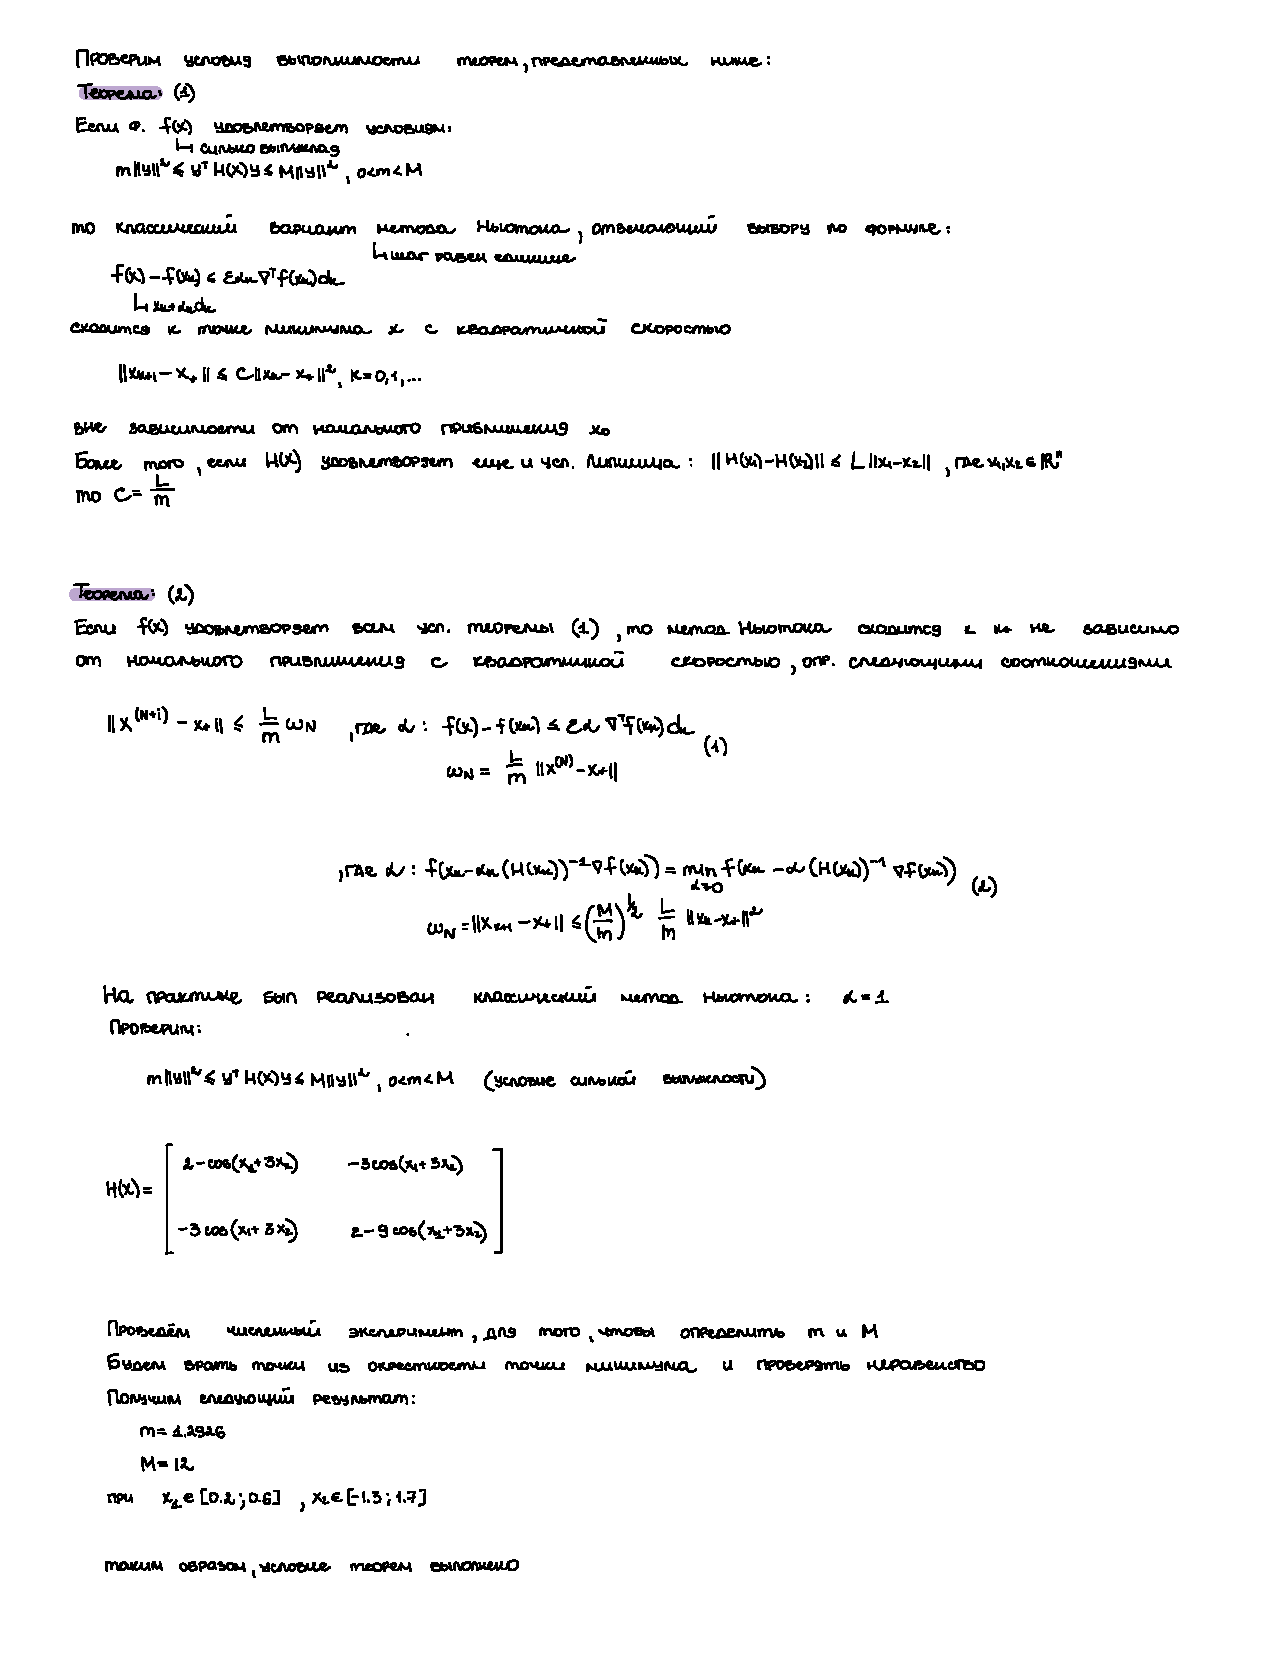
\includepdf[pages=-]{newton.pdf}
\section{Результаты решения задачи}
\section{Оценка достоверности результата}

\begin{thebibliography}{99}
	\bibitem{boldirev} Методы оптимизации. Математическое программирование: учеб. пособие. / Ю.Я. Болдырев, Е.А. Родионова; С.-Петерб. гос. техн. ун-т. - СПб.: Изд-во СПбГТУ, 1999. -- 81 с.: ил.
	% \bibitem{karmanov} Карманов, В.Г. Математическое программирование: Учеб. пособие. -- 6-е изд., испр. -- М.: ФИЗМАТЛИТ, 2008. -- 264 с. % yet unused
	% \bibitem{galeev} Галеев, Э. М., Тихомиров, В. М. Оптимизация: теория, примеры, задачи. -- М.: Эдиториал УРСС, 2000. -- 320 с. % yet unused
\end{thebibliography}

\end{document}